% -*-cap2.tex-*-
% Este fichero es parte de la plantilla LaTeX para
% la realización de Proyectos Final de Carrera, protegido
% bajo los términos de la licencia GFDL.
% Para más información, la licencia completa viene incluida en el
% fichero fdl-1.3.tex

% Copyright (C) 2009 Pablo Recio Quijano 

\section{Obtener Dominous}

Dominous se puede descargar desde varias fuentes principales. Dado que el lenguaje es interpretado y no compilado, el código
es válido tanto para sistemas basados en GNU/Linux como para Windows 7. \\

La descarga se puede hacer desde la web oficial~\cite{website:dominous} o desde los repositorios alojados en la 
forja de Rediris , en el que además del código fuente se cuenta con
herramientas como foros de consulta, descarga de manuales, bug tracker y otros.

\begin{figure}[h]
  \begin{center}
    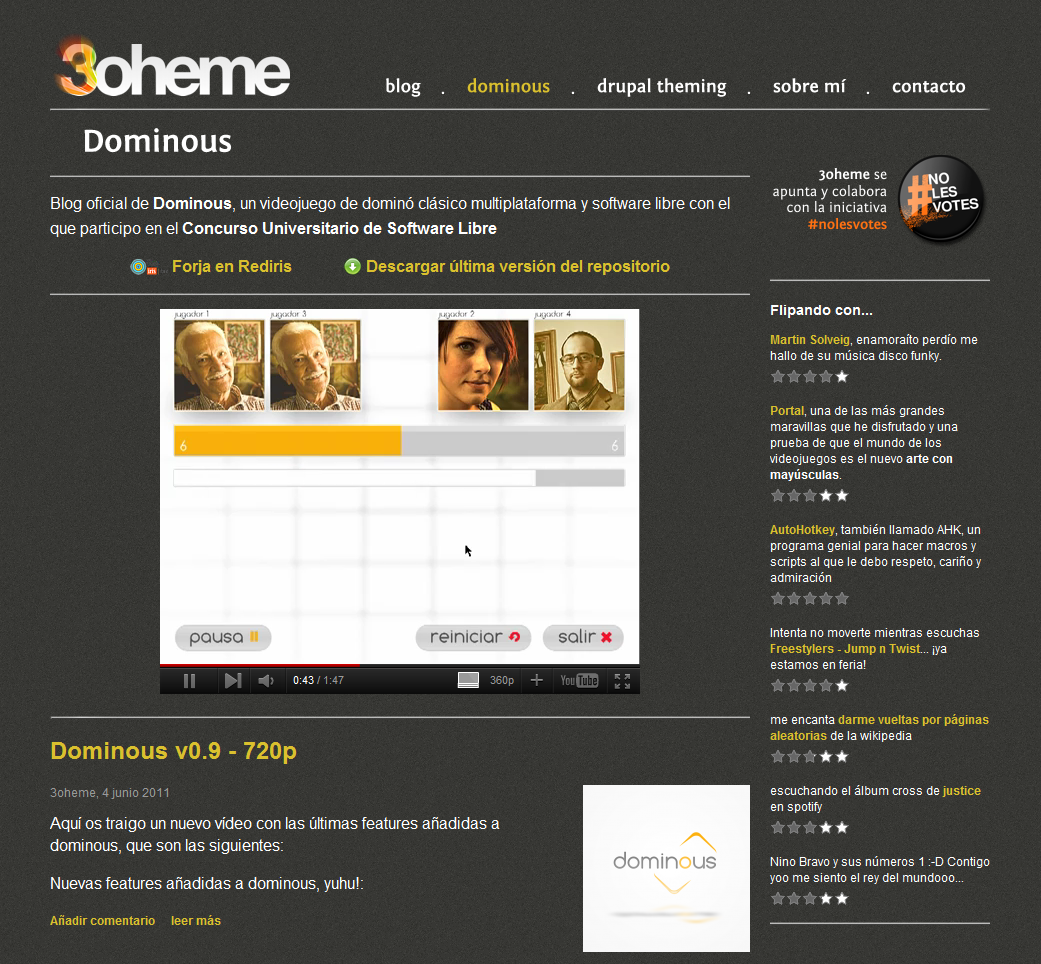
\includegraphics[scale=0.65]{pagina_oficial_dominous.png}
  \end{center}
  \caption{Página oficial de Dominous}
  \label{fig:pagina_oficial_dominous}
\end{figure}

\section{Instalación y ejecución en GNU/Linux}

La instalación bajo sistemas GNU/Linux requiere de cierto número de dependencias, que pueden ser instaladas cómodamente
con el siguiente comando:

\begin{lstlisting} [caption={Instalación de dependencias}, language=Bash, numbers=left]
user@machine:~$ sudo aptitude install python-pygame
                    python-setuptools && sudo easy_install
                    PyOpenGL PyOpenGL-accelerate
\end{lstlisting}

Como vemos, las dependencias que requiere la aplicación son las siguientes:

\begin{itemize}
    \item python-pygame
    \item python-setuptools
    \item PyOpenGL
    \item PyOpenGL-accelerate
\end{itemize}

Por último, para ejecutar y disfrutar de Dominous, solamente debemos acceder al directorio y ejecutar:

\begin{lstlisting} [language=Bash, numbers=left]
user@machine:~$ python dominous.py
\end{lstlisting}

\section{Instalación y ejecución en Windows}

Por otra parte, si deseamos instalar la aplicación en un sistema Windows, debemos ejecutar los siguientes pasos:

\begin{itemize}
    \item Obtener e instalar Python --- Para ello nos dirigimos a la página oficial de Python,
        descargamos la última versión estable (que en el momento de escribir este documento era la 2.7.2) y seguimos los pasos
        de instalación.
    \item Obtener e instalar PyOpenGL --- descargamos la última versión desde la página oficial de
        PyOpenGL y seguimos los pasos necesarios hasta instalarla
        correctamente en nuestro sistema.    
\end{itemize}

Para finalizar, nos dirigimos a la carpeta de Dominous y hacemos doble click sobre el icono de \comando{dominous.py}.
